\documentclass[12pt]{article}
\usepackage[a4paper, margin=.30in]{geometry}
\usepackage{graphicx ,
            wrapfig,
            xcolor, 
            enumerate,
            amsmath,fontenc
            }

\newcommand\headerMe[2]{\noindent{}#1\hfill#2}
\renewcommand{\thesection}{\Roman{section}}

\title{Leçon N 6 : Le mouvement}
\author{Zakaria HAOUZAN}
\date{\today}

\begin{document}
% headers --------------
\headerMe{Matière : Physique-Chimie}{Professeur : Zakaria HAOUZAN}\\
\headerMe{Unité : Travail Mécanique et Energie }{Établissement : Lycée SKHOR qualifiant}\\
\headerMe{Niveau : 1BAC-SM-X}{Heure : 6H}\\

% ------Content ________
\begin{center}

    \Large{Leçon $N^{\circ} 7 $: \color{red} ÉNERGIE CINÉTIQUE ET TRAVAIL}
\end{center}
\section{ Introduction : }
Immédiatement après son décollage , la navette spatiale reçoit une énergie cinétique croissante . Cette énergie dépend aussi de la
masse de la navette

Qu’est - ce que l’énergie cinétique d’un corps solide ? Quelle est
la relation existe entre le travail des forces exercées et l’énergie
cinétique ?
\section{Énergie cinétique : }
\subsection {Énergie cinétique d’un corps solide en translation  : }

Tout corps en mouvement possède une énergie cinétique note Ec
\\En mécanique, les énergies sont associées au mouvement, au déplacement dans l'espace, au changement produit.
La première d'entre elles, l'énergie cinétique, est fonction de la vitesse.
Elle est due au mouvement (anciennement "force vive") et existe en présence ou non de forces : selon que l'énergie varie ou non au cours du temps.

L’énergie cinétique Ec d’un point matériel de masse m et de vitesse instantanée v , est une grandeur scalaire toujours positive est définie par : $$E_c  = \frac{1}{2}mv^2$$

L’unité de l’énergie cinétique dans SI est le joule (J) .
La masse en (kg) et la vitesse en (m/s) .


\subsection{Énergie cinétique d’un corps solide en rotation autour d’un axe fixe  :}

\begin{wrapfigure}[18]{r}{0.3\textwidth}
    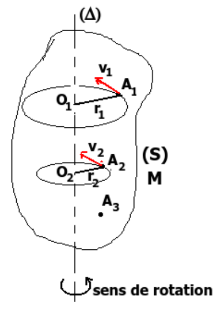
\includegraphics[width=0.25\textwidth]{./img/img01.png}
\end{wrapfigure}

Soit (S) un solide indéformable de masse totale M en mouvement de
rotation autour d’un axe fixe $(\Delta)$ de vitesse angulaire $\omega$ . Chaque point
de solide $A_i$ a une vitesse linéaire $v_i$ et de masse $m_i$
donc il possède une énergie cinétique: $E_{ci} = \frac{1}{2}m_iv^2_i$.

On sait que chaque vitesse linéaire $v_i = r_i.\omega$ avec $r_i$ le rayon de la trajectoire circulaire du point $A_i$. Donc l’énergie cinétique du point $A_i$ s’écrit : 
$$E_{ci} = \frac{1}{2}m_ir^2_i.\omega^2_i$$
D’où l’énergie cinétique totale du solide : 
$$E_{ci} = \sum_{i = 1}^n E_{ci} = \sum_{i = 1}^n\frac{1}{2}m_ir^2_i.\omega^2_i$$
$$E_{ci} = \frac{1}{2}.\omega^2_i\sum_{i = 1}^nm_ir^2_i$$

La grandeur $\sum_{i = 1}^nm_ir^2_i$ caractérise le solide (S) . Il dépend de sa masse et la répartition de cette masse autour de l’axe de rotation , cette grandeur est appelée : 

moment d’inertie du solide par rapport à l’axe $\Delta$ , son unité  dans le système international est $kg.m^2$ et on la note $J_{\Delta}$.
Donc $J_{\Delta} = \sum_{i = 1}^nm_ir^2_i$

\subsubsection {Définition : }
Énergie cinétique d’un corps solide en rotation autour d’un axe fixe, s’écrit : $$E_{c} = \frac{1}{2}J_{\Delta}\omega^2$$
avec $\omega$ la vitesse angulaire instantanée du solide et $J_{\Delta}$ le moment d’inertie du solide par rapport à l’axe de rotation ($\Delta$)
\subsubsection{Quelques moments d’inertie des solides homogènes et de formes connues :}
\begin{center}
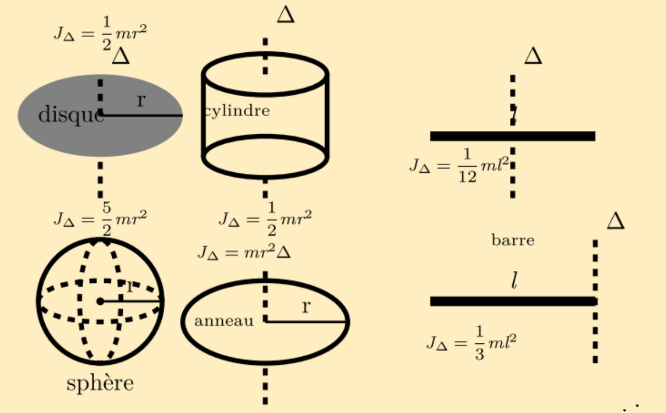
\includegraphics[width=0.50\textwidth]{./img/img00.png}
\end{center}
\subsubsection{Application : }
Une roue de 18kg et de $40cm$ de diamètre tourne à la fréquence de
rotation de 1500tr/min.

1. Calculer la vitesse linéaire d’un point de sa circonférence.

2. Déterminer son moment d’inertie et son énergie cinétique.

\section{Théorème de l’énergie cinétique : }
\subsection{Cas d’un corps solide en mouvement de translation sur un plan
incliné : }
Sur une table à coussin d’air ,inclinée d’un angle $\alpha = $10◦ par rapport au plan horizontale . De l’extrémité du banc , on
lâche un mobile autoporteur A de
masse m = 700g sans vitesse
initiale et on enregistre le mouvement du point G pendant des intervalle de temps successifs et égaux $\tau$ = 60ms . On obtient l’enregistrement suivant :
\begin{center}
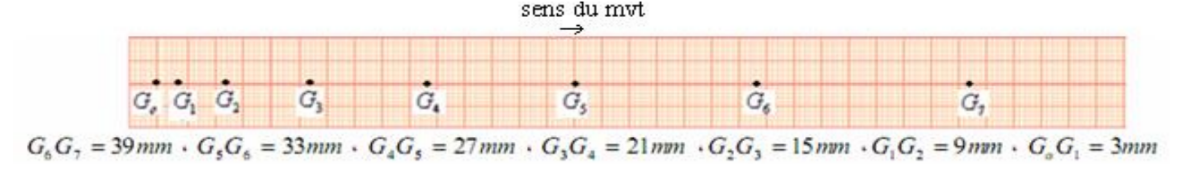
\includegraphics[width=1\textwidth]{./img/img02.png}
\end{center}


1) Donner le bilan des forces qui s'exercent sur l'autoporteur puis représenter les (sans échelle).\\
2) Donner l'expression du travail de chacune des forces qui s'exerce sur l'autoporteur entre G1 et G5 puis calculer la la somme des travaux des forces entre ces deux points.\\
3) Calculer l'énergie cinétique de l'autoporteur dans chacune des positions G3 et G5.\\
4) Calculer la variation de l'énergie cinétique : $\Delta E_c = E_{c5} - E_{c3} $\\
5) Comparer la somme des travaux des forces , quelle est votre conclusion? On prend g=9,8N/kg.

\subsection{Enoncé du théorème de l'énergie cinétique: }
Dans un repère Galiléen , la variation de l'énergie cinétique d'un corps solide en mouvement translation ou en mouvement de rotation autour d'un axe fixe ,entre deux instants ,est égale à la somme des travaux des forces appliquées sur ce corps entre ces deux instants.
$$\Delta E_c = \sum W(\vec{F})$$
$$\Delta E_c = E_{cf} - E_{ci}$$
Pour le Mouvement  de translation :  $$\Delta E_c = \frac{1}{2}mv_f^2 - \frac{1}{2}mv_i^2$$
\\Pour le Mouvement  de rotation    :  $$\Delta E_c = \frac{1}{2}J_{\Delta}.\omega^2_f - \frac{1}{2}J_{\Delta}.\omega^2_i$$


\end{document}

